\documentclass[PhD-Yoann-Dupont.tex]{subfiles}
\begin{document}

Comme nous l'avons vu dans le chapitre \ref{chap:NER-corpus}, il est difficile d'obtenir des corpus annotés en entités nommées. Lorsque ces corpus sont disponibles, il est également difficile d'obtenir des estimations de la qualité des annotations produite car les accords inter-annotateurs ne sont pas toujours calculés, par manque de temps ou de main d'\oe uvre, ou utilisent des métriques imprécises. En plus de l'utilisation d'outils adaptés, il existe des techniques d'apprentissage automatique permettant d'accélérer le processus d'annotation.

L'\textit{active learning} (apprentissage actif) \citep{angluin1987learning,kinzel1990improving,baum1991neural,mackay1992information}, est un type d'apprentissage semi-supervisé, dans lequel sont utilisés autant des données annotées que non annotées. L'apprentissage actif repose sur le principe qu'un apprenant (ici, un algorithme d'apprentissage automatique) est capable de requêter un oracle afin d'obtenir la sortie véritable sur de nouvelles données non annotées. Dans ce type d'apprentissage, nous avons typiquement un grand volume de données non annotées et très peu voire pas du tout de données annotées. L'\textit{apprentissage actif} est souvent utilisé dans le cas où le coût d'annoter de nouvelles données est important ou que les données annotées sont inexistantes malgré une tâche connue. Cette méthode permet d'accélérer le processus d'annotation ou de réduire le volume de données nécessaire à accomplir une tâche données. L'oracle est généralement un être humain, mais il peut également être une annotation de référence déjà connue dans le cas où l'on cherche à mesurer la vitesse d'annotation ou le volume de données minimum nécessaire. Le principe général de l'\textit{apprentissage actif} se résume dans une boucle dans laquelle l'apprenant va annoter des données inconnues et proposer les exemples les plus pertinents à l'oracle afin d'enrichir le jeu de données annotées. Une illustration schématique de l'apprentissage actif est disponible dans la figure \ref{fig:active-learning-loop}.

\begin{figure}[ht!]
\centering
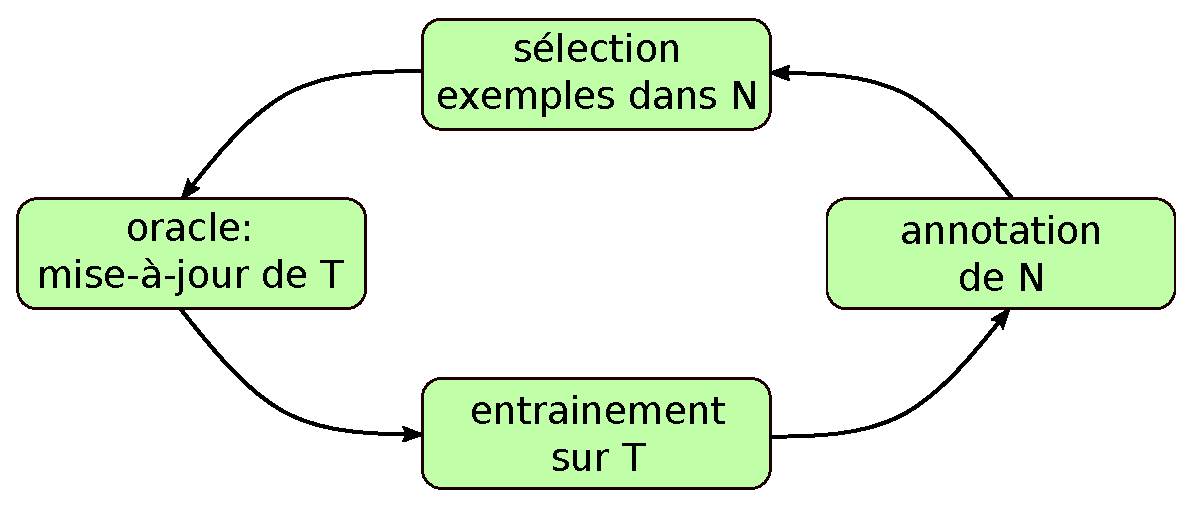
\includegraphics[scale=0.65]{images/active-learning/active-learning-loop}
\caption{Boucle d'\textit{active learning}.}
\label{fig:active-learning-loop}
\end{figure}

La sélection des exemples les plus pertinents est le point crucial de l'\textit{apprentissage actif}, qui influencera le nombre d'exemples nécessaires et donc la vitesse avec laquelle un corpus annoté suffisamment informatif pour l'algorithme d'apprentissage automatique sera créé. Il existe diverses stratégies pour effectuer cette tâche, parmi lesquelles nous pouvons citer :

\begin{itemize}
    \item sélection par densité d'information \citep{settles2008analysis}, où les exemples choisis sont ceux qui sont les plus différents de ceux déjà observés par le passé.
    \item sélection par incertitude \citep{lewis1994sequential}, où les exemples choisis sont ceux où l'apprenant est le plus incertain de ses décisions.
    \item sélection selon un comité \citep{mamitsuka1998query}, où un ensemble d'apprenants est utilisé. Les exemples choisis sont ceux où les différents apprenants sont le plus en désaccord les uns avec les autres.
    \item sélection par changement attendu du modèle, où les exemples choisis sont ceux qui ont le plus grand potentiel d'apporter des changements importants au modèle. Le critère de densité d'information \citep{settles2008analysis}, par exemple, sélectionne les exemples qui sont les plus différents de ceux déjà observés par le passé. \citet{claveau2017strategies} propose quant à lui une méthode adaptés aux CRF, se basant sur la proportion des features (le nombre N de features apparaissant X fois), les phrases sélectionnées étant celles permettant de plus se rapprocher de la répartition des fonctions caractéristiques déjà observées.
\end{itemize}

L'intérêt de l'apprentissage actif est multiple. Premièrement, il permet l'accélération du processus d'annotation en proposant des annotations candidates aux annotateurs humains qui peuvent simplement les corriger plutôt que de devoir les créer. Bien évidemment, dans le cadre de la reconnaissance des entités nomémes, toutes les annotations ne sont pas retrouvées par l'algorithme d'apprentissage, mais il est largement observé que le processus d'annotation en devient moins coûteux. Il est généralement reconnu que les systèmes entraînés en suivant une procédure d'apprentissage actif atteignent une meilleure qualité avec moins de données \citep{settles2011theories}. Ce gain de vitesse et cette réduction de la quantité de données requises pour une meilleure qualité laisse également supposer plus de possibilités pour le calcul d'un accord inter-annotateurs, et que cet accord sera plus important, ce qui laisse croire à une meilleure qualité de l'annotation.

Il a également été montré que l'apprentissage actif permet d'annoter avec plus de facilité les langues peu dotées \citep{garrette2013real}. Cette méthode semble donc aller particulièrement de pair avec l'apprentissage automatique de manière générale, dont la force est la grande adaptativité.

Dans le cadre de la reconnaissance des entités nommées, où il est difficile d'obtenir des données annotées et une évaluation de ces annotations, l'apprentissage actif est une piste de recherche sérieuse qui permettrait d'améliorer grandement la quantité et la qualité des corpus disponibles. Cela permet également d'envisager la production de corpus dans des langues peu dotées, pour lesquelles des ressources sont particulièrement difficiles à obtenir.

À notre connaissance, il n'existe aucune méthode par apprentissage actif qui soit étudiée pour effectuer de l'annotation structurée, les méthodes existantes supposent en effet une annotation non structurée. Or, comme nous l'avons vu, il est presque impossible de se passer de toute forme de structuration dans le cadre de la reconnaissance des entités nommées. La structuration des entités nommées pose des questions intéressantes dans le cadre de l'apprentissage actif. Par exemple, quelles annotations doit montrer l'algorithme ? Reprenons l'exemple de la figure \ref{fig:address-tree}. L'approche la plus immédiate serait de faire annoter à l'utilisateur des arbres entiers. Cette approche a cependant le problème d'être particulièrement longue dans les premières itérations. Nous avons également vu que le problème principal des méthodes par apprentissage demeurait le silence, ce qui laisse supposer plus de travail du côté de l'annotateur, donc une annotation moins rapide.

Peut-on imaginer une procédure alternative pour annoter plus rapidement dans un premier temps ? Nous pourrions supposer que l'utilisateur n'annote d'abord que les composants les plus simples et que un système à base de règles puisse donner des suggestions, même bruitées ? Pour l'exemple de la figure \ref{fig:address-tree}, il est tout à fait envisageable de n'annoter que les composants qui constituent les feuilles de l'arbre et d'appliquer ensuite des règles simples pour reconstruire l'arbre entier et le proposer à l'utilisateur pour validation. Lorsqu'un certain nombre d'exemples simples auront été annotés, nous pourrions alors repasser à une manière plus classique d'annoter. La suggestion de cette annotation pourrait même se faire au moment de l'annotation : par exemple, lorsqu'un prénom suivi d'un nom sont annoté, le système pourrait automatiquement proposer une annotation de personne les recouvrant tous les deux. Beaucoup d'entités nommées structurées sont régies par des règles simples, la suggestion au moment de l'annotation permettrait aux annotateurs d'aller beaucoup plus vite. Même si ces suggestions ne peuvent pas être systématiquement faites, il semble improbable qu'elles ralentissent le processus d'annotation.

Lorsque des arbres doivent être annotés, se pose également la question de comment les annoter. Doit-on annoter de manière \emph{top-down} (de la racine aux feuilles) ou de manière \emph{bottom-up} (des feuilles à la racine) ? Dans le cas des annotations Quaero, certains composants sont difficiles à identifier de prime abord (typiquement ceux ayant les plus grands manques à gagner dans le tableau \ref{tab:fscore-shortfalls}), mais le sont plus simplement une fois les entités qui les recouvrent identifiées. Parmi les travaux déjà effectués sur l'apprentissage actif d'annotations structurées, nous pouvons citer \citet{hwa2004sample} propose de nombreux critères pour la sélection de nouveaux exemples non-annotés. Nous pouvons aussi citer \citet{baldridge2004active}, qui propose un critère de réutilisabilité des annotations par d'autres modèles afin de réduire la quantité d'annotations.

De manière générale, l'apprentissage actif pour les entités nommées structurées pose différentes questions lorsqu'elle doit être effectuée par un être humain (plutôt que simulé par une machine). L'humain doit-il annoter complètement les entités structurées ? Comment l'être humain trouve-t-il plus naturel d'annoter ? Doit-on concevoir des approches spécifiques pour l'apprentissage actif des entité nommées structurées ? Il semble difficile de répondre à ces questions sans tester de manière empirique les différentes approches. Nous entendons étudier cette problématique à l'avenir qui soulève différentes questions et pour lesquelles des éléments de réponse pourraient rendre plus simple la constitution de données annotées à la qualité plus certifiable.

\end{document}